% !TEX root = /Users/kquine/Dropbox/Research/Papers/2015/CPS-SMT-RTSS/cps-rtss.tex

%
\section{Case Studies and Experimental Results}
\label{sec:case-studies}

This section gives an overview of some 
case studies using Hybrid PALS and SMT-based analysis to verify %and experimental results 
distributed CPSs. 
%
These case studies involve nontrivial (nonlinear) ODEs,
due to the  continuous physical interaction between distributed components.
We have verified safety properties 
using %bounded reachability, 
inductive and compositional SMT encodings
for \emph{any possible} set of  local clocks  maximal clock skew $\epsilon$.
%
All  experiments in this section
were conducted on an Intel Xeon 2.0 GHz with 64 GB memory.
%running 64-bit Ubuntu 12.04.5 LTS.
%We set a timeout of 30 hours. % for the experiments.
The case studies and the experimental evaluation are available at %the
%\textsf{dReal} tool webpage
\url{http://dreal.github.io/benchmarks/networks}. 




\subsection{Turning an Airplane}
\label{sec:ex-airplane}

We consider a multirate distributed CPS
to turn an airplane (adapted from \cite{ftscs-journal}).
%in which a \emph{main controller} directs \emph{subcontrollers} for the ailerons and the rudder in a synchronous way.
%
To make a turn, an aircraft rolls towards the direction of the turn
by moving its \emph{ailerons} % (surfaces attached to the end of the wings).
The rolling causes 
a yawing moment in the opposite direction, called \emph{adverse yaw},
which is countered by using its \emph{rudder} (a surface attached to the vertical stabilizer).
%
The subcontrollers for the ailerons and the rudder operate at different rates, 
and the main controller orchestrates them to achieve a smooth turn.
%
Fig.~\ref{fig:airplane-ctrl} illustrates the multirate ensemble $\mathcal{E}$ of our system.


\begin{figure}
\centering
\tikzstyle{comp}=[draw,thick,rounded corners=4pt,text centered]
\tikzstyle{env}=[draw,dashed,rounded corners=8pt,text centered]
\tikzstyle{conn}=[thick,-latex,font=\scriptsize]
\tikzstyle{envconn}=[very thin,-open triangle 45,font=\scriptsize]
\begin{tikzpicture}[scale=0.9,every node/.style={transform shape},font=\footnotesize]
%components
\node (main) [comp,text width=8ex,minimum height=13ex] {{Main} ($60\, \mathrm{ms}$, $\mathit{rate}$ = $1$)}; 
\path (main.east) + (16ex,8ex) node (left) [comp,text width=14ex] {{Left aileron} ($15\,\mathrm{ms}$, $\mathit{rate}$ = $4$)}; 
\path (main.east) + (16ex,1.3ex) node (vert) [comp,text width=14ex] {{Rudder}\\ ($20\, \mathrm{ms}$, $\mathit{rate}$ = $3$)}; 
\path (main.east |- main.-48) + (16ex,0ex) node (right) [comp,text width=14ex] {{Right aileron} ($15\,\mathrm{ms}$, $\mathit{rate}$ = $4$)}; 
%comp connections
\draw [conn,latex-] (main.west |- main.north) + (3ex,0)-- node{ }+(3ex,2ex) node[above] {$\mathit{goal}_\psi$};
\draw [conn] (main.east |- main.north) + (-3ex,0)-- node{ }+(-3ex,2ex) node[above] {$\psi$};
\draw[conn] ($(main.48)+(0,0.5ex)$) -- node[above,sloped] {$\mathit{goal}_L$} ($(left.west |- left)+(0,0.5ex)$);
\draw[conn] ($(left.west |- left)+(0,-0.5ex)$) -- node[below,sloped] {$v_L$} ($(main.48)+(0,-0.5ex)$);
\draw[conn] ($(main.east)+(0,0.5ex)$) -- node[above,sloped] {$\mathit{goal}_V$} ($(vert.west |- vert)+(0,0.5ex)$);
\draw[conn] ($(vert.west |- vert)+(0,-0.5ex)$) -- node[below,sloped] {$v_V$} ($(main.east)+(0,-0.5ex)$);
\draw[conn] ($(main.-48)+(0,0.5ex)$) -- node[above,sloped] {$\mathit{goal}_R$} ($(right.west |- right)+(0,0.5ex)$);
\draw[conn] ($(right.west |- right)+(0,-0.5ex)$) -- node[below,sloped] {$v_R$} ($(main.-48)+(0,-0.5ex)$);
%physical envs
\path (main.west) + (-8ex,0ex) node (main-env) [env,text width=6ex,minimum height=13ex] {$E_\mathit{Main}$}; 
\path (left.east) + (12ex,0ex) node (left-env) [env,text width=7ex,minimum height=5ex] {$E_\mathit{Left}$}; 
\path (vert.east) + (12ex,0ex) node (vert-env) [env,text width=7ex,minimum height=5ex] {$E_\mathit{Rudder}$}; 
\path (right.east) + (12ex,0ex) node (right-env) [env,text width=7ex,minimum height=5ex] {$E_\mathit{Right}$}; 
%physical env conns
\draw[envconn] ($(main-env.east)+(0,4.5ex)$) -- node[above] {$\psi$} ($(main.west |- main-env)+(0,4.5ex)$);
\draw[envconn] (main-env.east) -- node[above] {$\phi$} (main.west);
\draw[envconn] ($(main-env.east)+(0,-4.5ex)$) -- node[above] {$\beta$} ($(main.west |- main-env)+(0,-4.5ex)$);
\draw[envconn] ($(left.east |- left-env)+(0,0.5ex)$) -- node[above] {$\mathit{rate}_L$} ($(left-env.west |- left-env)+(0,0.5ex)$);
\draw[envconn] ($(left-env.west |- left-env)+(0,-0.5ex)$) -- node[below] {$\alpha_L$} ($(left.east |- left-env)+(0,-0.5ex)$);
\draw[envconn] ($(vert.east |- vert-env)+(0,0.5ex)$) -- node[above] {$\mathit{rate}_\mathit{V}$} ($(vert-env.west |- vert-env)+(0,0.5ex)$);
\draw[envconn] ($(vert-env.west |- vert-env)+(0,-0.5ex)$) -- node[below] {$\alpha_V$} ($(vert.east |- vert-env)+(0,-0.5ex)$);
\draw[envconn] ($(right.east |- right-env)+(0,0.5ex)$) -- node[above] {$\mathit{rate}_\mathit{R}$} ($(right-env.west |- right-env)+(0,0.5ex)$);
\draw[envconn] ($(right-env.west |- right-env)+(0,-0.5ex)$) -- node[below] {$\alpha_R$} ($(right.east |- right-env)+(0,-0.5ex)$);
\end{tikzpicture}
\caption{The distributed controllers for turning an airplane.} \label{fig:airplane-ctrl}
\end{figure}


Each subcontroller $M$ gradually moves its surface towards the goal
angle $\mathit{goal}_M$ specified by the main controller
$M_\mathit{Main}$. 
In each round, $M$ receives $\mathit{goal}_M$ from $M_\mathit{Main}$,
determines the moving rate $\mathit{rate}_M$ based on $\mathit{goal}_M$ 
and the current sampled value $v_M$ of the surface angle $\alpha_M$,
and sends back $v_M$ to $M_\mathit{Main}$
(e.g., the new value of $\mathit{rate}_M$ can be given by
$ \sign(\mathit{goal}_M - v_M) \cdot \min(\abs(\mathit{goal}_M - v_M) / T, \mathit{max}_M)$).
The continuous dynamics of $\alpha_M$ is specified 
by the local physical environment $E_M$
as the ODE $\frac{\mathrm{d}\alpha_M}{\mathrm{d}t} = \mathit{rate}_M$.
%\footnote{$E_M$ is the controlled physical environment $E_M = (\mathbb{R}, \alpha_M, \Lambda_M)$
%with $((\mathit{rate}_M,T,v_M),\tau) \in \Lambda_M$ iff 
%$\tau(t) = v_M + \int_0^t  \mathit{rate}_M \,\mathrm{d}t$ for $t \in [0, T]$.}

The main controller $M_\mathit{Main}$ determines the goal angles for the subcontrollers to make a coordinated turn.
In  each round, $M_\mathit{Main}$ receives a  desired direction $\mathit{goal}_\psi$ %of the airplane 
(from the pilot)
and the surface angles $(v_L, v_V, v_R)$ from the subcontrollers, 
and then sends back the new goal angles $(\mathit{goal}_L,\mathit{goal}_V,\mathit{goal}_R)$,
%to the subcontrollers,
based on the current sampled \emph{position} values $(v_\psi, v_\phi, v_\beta)$ 
of  the direction angle $\psi$, the roll angle $\phi$, and the yaw angle $\beta$.


We consider a simple control logic to decide 
the new goal angles $(\mathit{goal}_L,\mathit{goal}_V,\mathit{goal}_R)$,
by three control functions \cite{ftscs-journal}:
%
\begin{inparaenum}[(i)]
	\item $f_\phi(v_\phi, v_\psi, \mathit{goal}_\psi)$
		returns the goal roll angle $\mathit{goal}_\phi$,
		%based on the sampled roll angle $v_\phi$, the sampled direction $v_\psi$, 
		%and the goal direction $\mathit{goal}_\psi$;
	\item $f_{R}(v_\phi, \mathit{goal}_\phi)$ returns the goal angle $\mathit{goal}_R$ for the right aileron
	(where the goal angle $\mathit{goal}_L$ for the left aileron is the opposite angle $- \mathit{goal}_R$);
	%the left aileron angle is %always  exactly opposite to the right aileron angle); 
	and
	\item $f_V(v_\beta)$ returns the goal rudder angle $\mathit{goal}_V$.
	%based on the sampled yaw angle $v_\beta$. % (the goal yaw angle is $0^\circ$).
\end{inparaenum}
For example, for $h = 0.32  (\mathit{g}_\psi - v_\psi)$:
\begin{align*}
f_\phi(v_\phi, v_\psi, g_\psi) &= 
v_\phi + \sign(h - v_\phi) \cdot \min(\abs(h - v_\phi),1.5)
\\
f_{R}(v_\phi, g_\phi) &=
\sign(\mathit{g}_\phi - v_\phi)\cdot \min(0.3 \,\abs(\mathit{g}_\phi - v_\phi), 45))
\\
f_V(v_\beta) &=
\sign(-v_\beta)\cdot \min(0.3  \,\abs(v_\beta), 30).
\end{align*}

In the physical environment $E_\mathit{Main}$,
the lateral dynamics of an aircraft
can be specified as the following nonlinear ODEs,
where $p$ is the rolling moment, $r$ is the yawing moment,
and $Y_{\delta_L,\delta_V,\delta_R,\beta}$, $L_{\delta_L,\delta_V,\delta_R,\beta}$, and $N_{\delta_L,\delta_V,\delta_R,\beta}$
are (linear) functions of the control angles $(\delta_L,\delta_V,\delta_R)$ 
%for the ailerons and the rudder
and $\beta$
%respectively denoting  the coefficients of side force, rolling moment, and yawing moment.
\cite{stevens2003aircraft}:
%
\begin{align*}
\dot{\beta} &= Y_{\delta_L,\delta_V,\delta_R,\beta} / m V - r + (g / V) \cos \beta \sin \phi,
\\
\dot{\phi} &= p,
\qquad\qquad\qquad\qquad
\dot{\psi} = (g / V) \tan \phi,
\\
\dot{p} &= (c_1 r + c_2 p) \cdot r  \tan \phi + c_3 L_{\delta_L,\delta_V,\delta_R,\beta} + c_4 N_{\delta_L,\delta_V,\delta_R,\beta},
\\
\dot{r} &= (c_8 p - c_2 r)  \cdot r  \tan \phi + c_4 L_{\delta_L,\delta_V,\delta_R,\beta} + c_9 N_{\delta_L,\delta_V,\delta_R,\beta}.
\end{align*}
%


The physical environment $E_\mathit{Main}$ clearly depends on the subcontrollers's physical environments.
Each control angle $\delta_M$ in  $E_\mathit{Main}$ must be the same as the corresponding surface angle $\alpha_M$.
%
Such  immediate physical correlations between the local %physical 
environments are specified by the time-invariant constraint
%
\[\forall t.\, (\delta_L(t) = \alpha_L(t)) \wedge (\delta_V(t) = \alpha_V(t)) \wedge (\delta_R(t) = \alpha_R(t)).
\]
Notice that since the main controller and the subcontrollers have \emph{different periods with local clock skews},
the ODEs of the subcontrollers cannot be directly ``plugged'' into $E_\mathit{Main}$.
%%% (Peter)  The following can be skipped:
%The PALS models consist of the multirate ensemble $\mathcal{E}$, the physical environments, and the time-invariant constraint,
%along with appropriate  sampling and response timing policies $\Pi$.

The safety property of $\mathcal{E}$ 
is that the yaw angle $\beta$ is always close to $0$ (e.g., $\forall t.\; \beta(t) < 0.1$).
In the analysis,
we assume that the maximal clock skew is $\epsilon = 0.1\,\mathrm{ms}$,
the sampling time $t_I$ is $0\,\mathrm{ms}$ for every controller,
and the response time $t_R$ is $3\,\mathrm{ms}$ for the subcontrollers.
%(the main controller has no actuators).
%To verify the safety property $\forall t.\; \beta(t) < 0.1$ (without any time bound), 
%we consider the simple inductive condition $\Psi(\vec{z})$ with $\vec{z} = (\beta,\psi,p,r)$:
%\[
%|\beta| < 0.1
%\;\wedge\;
%|\psi| < 0.8
%\;\wedge\;
%|p| < 1
%\;\wedge\;
%|r| < 1.
%\]
%We have proved that $(\Psi(\vec{z}) \wedge \phi_{\mathcal{E} \restriction_{\Pi} E_\mathcal{E}}^{T,i}(\vec{z}\shortmid\vec{z'})) \rightarrow \Psi(\vec{z'})$
%and  $\Psi(\vec{z}) \rightarrow (\forall t \in [0,T].\; \beta(t) < 0.1)$ hold
%using \textsf{dReal} by checking the unsatisfiability of their negated formulas
%(i.e.,
% $\Psi(\vec{z}) \wedge \phi_{\mathcal{E} \restriction_{\Pi} E_\mathcal{E}}^{T,i}(\vec{z}\shortmid\vec{z'}) \wedge \neg \Psi(\vec{z'})$ and $\Psi(\vec{z}) \wedge \beta(t) \geq 0.1$).
%As a consequence, the safety property $\forall t.\; \beta(t) < 0.1$
%holds from any initial state satisfying $\Psi(\vec{z})$ for any local clocks.
\textbf{Working on the verification.}


\subsection{Networked Water Tank Controllers}

In this case study, adapted from
\cite{kowalewski1999case,raisch1999approximating}, 
a number of water tanks are connected by pipes as shown in
Figure~\ref{fig:water}.  \textbf{KYUNGMIN: I cannot see on Fig 8 that
  they are connected ...}
The water level in each tank is controlled by a pump in the tank, and 
 depends on the pump's mode $m \in \{m_\texttt{on}, m_\texttt{off}\}$
and the water levels of the adjacent tanks.
The water level $x_i$ of tank $i$ changes according to the ODEs:%
\footnote{%where 
$A_i, q_i, a, b $ are constants determined by the size of the tank, the power of the pump, 
and the widths of the I/O pipes,
and $g$ is the %standard 
gravity constant.}
\[
\begin{aligned}
A_i \dot{x}_i &=  (q_i + a \sqrt{2g} \sqrt{x_{i-1}})  - b \sqrt{2g} \sqrt{x_i}
&& \mbox{if}\;\; m_i = m_\texttt{on},
\\
A_i \dot{x}_i &= a \sqrt{2g} \sqrt{x_{i-1}}  - b \sqrt{2g} \sqrt{x_i}
&& \mbox{if}\;\; m_i = m_\texttt{off},
\end{aligned}
\]
We set $x_0 = 0$ for the leftmost tank $1$.
%
Every pipe controller performs its transitions according to its local
clock and sets  
the pump to on if $x_i \leq L_m$ and to off if $x_i > L_M$.

\begin{figure}
\centering
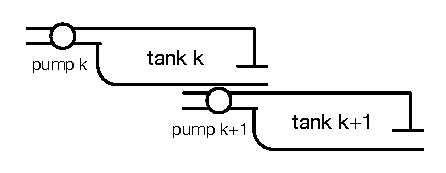
\includegraphics[clip=true,trim=0.3cm 0.35cm 0.3cm 0.35cm,width=0.6\columnwidth]{water.pdf}    
\caption{Connected water tanks.}  \label{fig:water}
\end{figure}

The safety property is that the water level of each tank is in a certain range
$I = [L_m - \eta, L_M + \eta]$.
%
We have verified this safety property for  \emph{any number} of connected water tanks 
using inductive and compositional analysis.%
\footnote{For a tank $k$ and %a subinterval 
$I' = [L_m - \eta', L_M + \eta']\subseteq I$ with $\eta' < \eta$,
provided  that $x_{k-1} \in I$ always holds, % for its input tank  $k-1$.
we show that $x_{k} \in I'$ is an inductive condition,
and  $x_{k} \in I$ always holds
if $x_{k} \in I'$ at the beginning of each round
(i.e., $(x_k(0) \in I' \wedge \phi_{\mathcal{E} \restriction_{\Pi}
  E_\mathcal{E}}^{T,0}) \rightarrow (x_k(T) \in I') \wedge (\forall t
\in [0,T].\; x_{k}(t) \in I)$).} 
%
For  maximal clock skew $\epsilon = 30\,\mathrm{ms}$,
 sampling time $t_I = 20\,\mathrm{ms}$,
and  response time $t_R = 100\,\mathrm{ms}$,
we have proved the  compositional safety property
% for any number of water tanks
% by checking the unsatisfiability of the negated formulas,
 using \textsf{dReal} with precision $\delta = 0.001$ (the analysis took $4.3$ seconds).%
 \footnote{In the analysis, we use the parameters 
$a = 0.5$, $b = 0.6$, $g = 9.8$, $A = 2$, $q = 4$, $L_m = 8$, $L_M = 10$,
$\eta = 3$, $\eta' = 2$, and $T = 1\,\mathrm{s}$.}
However, if $\epsilon = 150\,\mathrm{ms}$,
then the compositional inductive condition is violated by the trajectory in Fig.~\ref{fig:water-error}
%generated by \textsf{dReal} with precision $\delta = 0.001$
(the analysis took $1.46$ seconds).

\begin{figure}
\centering
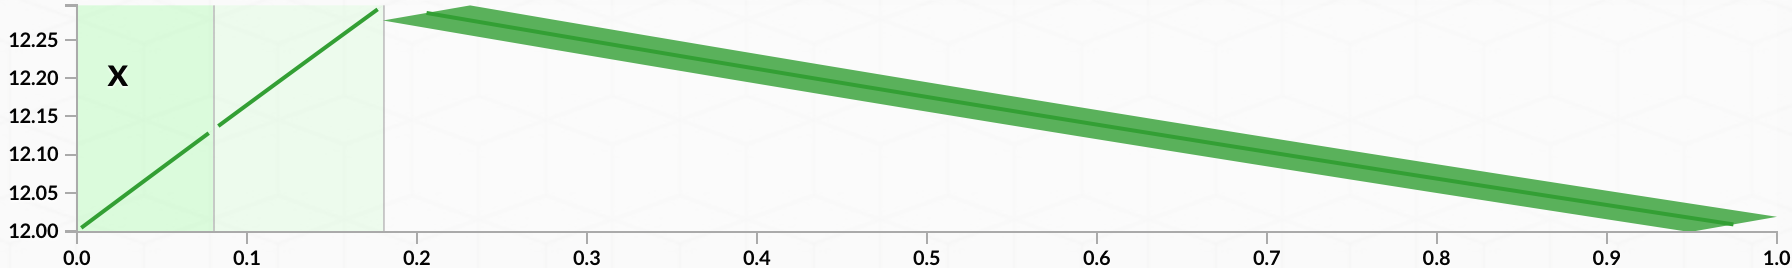
\includegraphics[clip=true,trim=1ex 1ex 1ex 1ex,width=\columnwidth]{water-error.png}    
\caption{The counterexample trajectory when $\epsilon = 150\,\mathrm{ms}$,
where the water level increases for extra $300\,\mathrm{ms}$ to violate the inductive condition. % at the end of the round.
} \label{fig:water-error}
\end{figure}





\subsection{Networked Thermostat Controllers}

%A classical thermostat controller  \cite{henzinger2000theory} is installed in each room.
%(where the specification of a single hybrid automaton is adapted from \cite{henzinger2000theory}). 
A number of rooms are interconnected by open doors, 
as shown in Fig.~\ref{fig:adj-rooms}.
The temperature of each room is separately controlled by its own
thermostat controller that turns the heater on and off.
That is, it %The temperature of each room 
depends on
the heater's mode $m \in \{m_\texttt{on}, m_\texttt{off}\}$  and the temperatures of the other rooms.
The temperature $x_i$ of room $i$
changes according to the ODEs:%
\footnote{%where 
$K_i, h_i \in \mathbb{R}$ are constants depending on
the size of room $i$ and the heater's power, respectively,
and $c \in \mathbb{R}$ is determined by the size of the open door.}
\begin{align*}
\dot{x}_i &= K_i (h_i - ((1- 2 c) x_i + c x_{i-1} + c x_{i+1})) &&\mbox{if}\; m_i = m_\texttt{on}
\\
\dot{x}_i &= - K_i ((1- 2 c) x_i + c x_{i-1} + c x_{i+1}) && \mbox{if}\; m_i = m_\texttt{off}
\end{align*}
%
In each transition, a controller turns on the heater 
 if $x_i \leq T_m$,
and turns it  off if $x_i > T_M$.

\begin{figure}
\centering
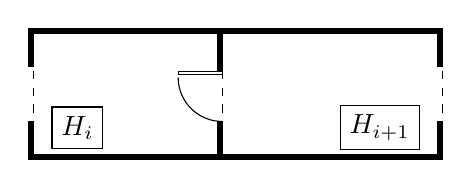
\begin{tikzpicture}[scale=0.8] %baseline=(current bounding box.north)
%left wall
\filldraw  (-3,0.08) rectangle  + (-0.08,-0.6)
	(-3,-2.0) rectangle  + (-0.08,0.6);
\draw[dashed] (-3,-0.6) -- (-3,-2);
%room1
\filldraw (0,0) rectangle  + (-3,0.08)
	(-3.08,-2.0) rectangle  + (3,0.08);
\path (-2.3,-1.5) node[draw] { $H_i$};
%wall
\filldraw (0,-0.6) rectangle  + (-0.08,0.6)
	(0,-2.0) rectangle  + (-0.08,0.6);
\draw[dashed] (0,-0.6) -- (0,-2);
%door
\draw (0,-0.6) rectangle +(-0.7,-0.05);
\draw (-0.7,-0.7) arc (180:270:0.7);
%room2
\filldraw (0,0) rectangle  + (3.5,0.08)
	(3.5,-2.0) rectangle  + (-3.5,0.08);
\path (2.5,-1.5) node[draw] (m2){ $H_{i+1}$};
%right wall
\filldraw  (3.5,0.08) rectangle  + (-0.08,-0.6)
	(3.5,-2.0) rectangle  + (-0.08,0.6);
\draw[dashed] (3.5,-0.6) -- (3.5,-2);
\end{tikzpicture}
\caption{Interconnected rooms. %  by an open door.
} \label{fig:adj-rooms}
\end{figure}

The safety property is that the temperature of each room
is in the range $I = [T_m - \eta, T_M + \eta]$.
We have verified the safety property $\forall t.\; x_i \in I$
for  \emph{any number} of interconnected thermostat controllers
by inductive and compositional analysis.%
\footnote{For %a subinterval 
$I' = [T_m - \eta', T_M + \eta']\subseteq I$,
provided that both $x_{i-1} \in I$ and $x_{i+1} \in I$ always hold,
we show that $x_i \in I'$ is an inductive condition,
and $x_i \in I$ always holds
if $x_i \in I'$ at the beginning of each round.}
%
For $\epsilon = 2\,\mathrm{ms}$,
$t_I = 10\,\mathrm{ms}$,
and $t_R = 200\,\mathrm{ms}$,
we have proved (in $2.6$ seconds) the compositional safety property 
%for any number of thermostats 
%by checking the unsatisfiability of the negated formulas,
 using \textsf{dReal} with precision $\delta = 0.001$.\footnote{In the analysis, we use the parameters $K = 0.015$, 
$h = 100$,
$c = 0.01$,
$T_M = 21$, 
$T_m = 19$,
$\eta = 3$, $\eta' = 2$,
and $T = 1\,\mathrm{s}$.}
%
However, if $\epsilon = 20\,\mathrm{ms}$,
then the compositional inductive condition is violated by the trajectory in Fig.~\ref{fig:thermo-error}
(the analysis took $0.56$ seconds).


\begin{figure}
\centering
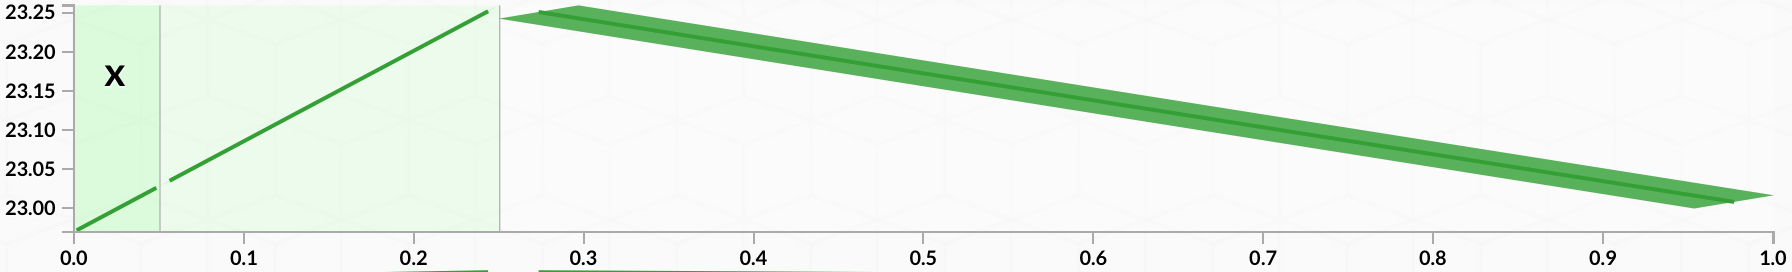
\includegraphics[clip=true,trim=1ex 1ex 1ex 1ex,width=\columnwidth]{thermo-error.png}    
\caption{The counterexample trajectory when $\epsilon = 20\,\mathrm{ms}$.
%where the temperature  rises for extra $20\,\mathrm{ms}$ and thus $x > 23$ at the end of the round.
} \label{fig:thermo-error}
\end{figure}


%\subsection{Automated Highway System}
%
%...

%\subsection{Quadrotor Attitude Controller}
%\label{sec:quadrotor}
%..

%\subsection{Steam Boiler Controller}
%...

\subsection{Bounded Reachability Comparison}
\label{sec:expr}

We have implemented the SMT algorithm
for our new logic $\mathcal{L}_{\mathcal{F}\cup\mathcal{N}}$ in the \textsf{dReal} SMT solver \cite{dReal},
and have compared the performance of 
the new $\mathcal{L}_{\mathcal{F}\cup\mathcal{N}}$-encoding
with one of the previous \emph{non-modular} $\mathcal{L}_{\mathcal{F}}$-encoding  for Hybrid PALS models.
%
In this comparison,
we only consider special cases %of the examples 
with no clock skews ($\epsilon = 0$) 
due to a lack of expressiveness of  $\mathcal{L}_{\mathcal{F}}$,
and only bounded reachability analysis
since it needs to generate bigger formulas than other types of analysis.


We have performed bounded reachability analysis up to $k = 5$
for the safety properties for the ``concrete'' instances of the case studies
(using \textsf{dReal} without the use of other SMT heuristics).
The results for $k$-step bounded reachability analysis 
are summarized  in Fig.~\ref{table:bounded} and show that
%
the new encoding significantly outperforms 
the non-modular encoding.\footnote{We consider both \texttt{unsat} (verified) and \texttt{sat}  (counterexample found) cases
by using different safety properties.}
For example, 
the SMT analysis using the non-modular encoding
for  three interconnected thermostats
 did not terminate for $30$ hours
even for $k = 2$.


\begin{figure}
\centering
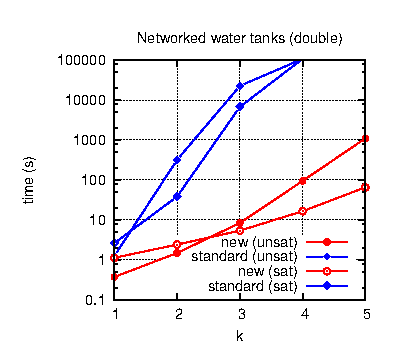
\includegraphics[width=0.45\columnwidth]{plot/water-double.eps}    
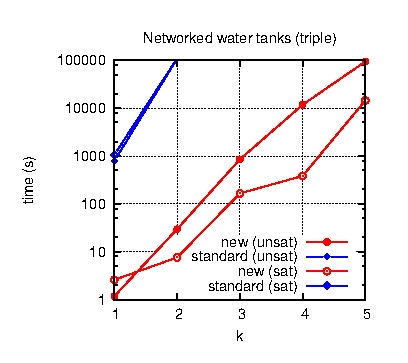
\includegraphics[width=0.45\columnwidth]{plot/water-triple.eps}    
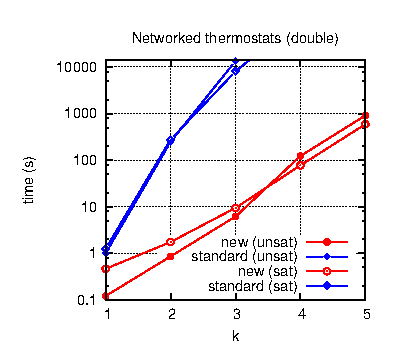
\includegraphics[width=0.45\columnwidth]{plot/thermostat-double.eps}    
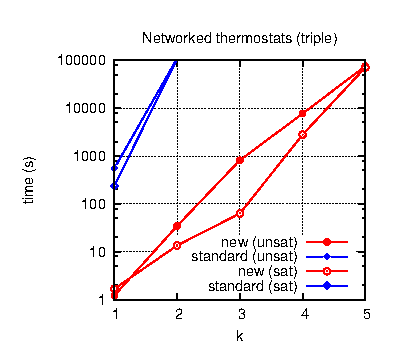
\includegraphics[width=0.45\columnwidth]{plot/thermostat-triple.eps}    
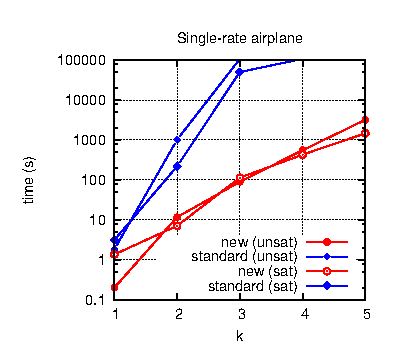
\includegraphics[width=0.45\columnwidth]{plot/airplane-single.eps}    
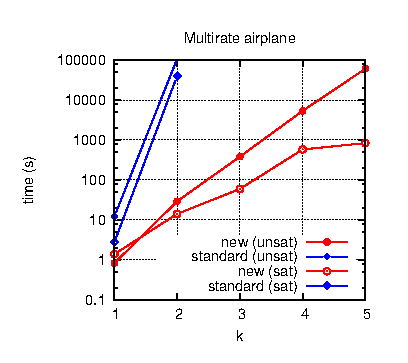
\includegraphics[width=0.45\columnwidth]{plot/airplane-multi.eps}    
\caption{Running time of $k$-step bounded reachability analysis, where red lines denote the new encoding,
and blue lines denote the non-modular encoding.}
\label{table:bounded}
\end{figure}





